\setchapterpreamble[u]{\margintoc}
\glsresetall % reset glossary
\chapter{Evaluating discretization approaches for ultralight structure optimization} \label{chp:03}
The process of topology optimization for a structure involves the selection and sizing of optimal elements within a predetermined set. As discussed in the previous chapter, in our context this set could be composed of either continuum elements (shell or volumetric) or truss-like elements. Based on the discretization choice we distinguish between density-based topology optimization and \gls{tto} \marginnote{Part of the content presented in this chapter has been published and showcased during a conference as:\\Stragiotti, E. et al. (2021) "Towards manufactured lattice structures: a comparison between layout and topology optimization", in \textit{AeroBest 2021 International Conference on Multidisciplinary Design Optimization of Aerospace Systems}. Book of proceedings. Lisbon, Portugal: ECCOMAS~\cite{stragiotti_towards_2021}.}. This chapter aims to assess the suitability and the inherent advantages and disadvantages of both methods when optimizing ultralight structures \ie structures that exhibit a low volume fraction, typically below 5\%. 

For this purpose, we initially formulate a volume minimization problem subject to maximum stress constraints for both discretizations in \secref{sec:03_common_prob}. Later, a two-dimensional test case, featuring identical dimensions, loads, and material properties is optimized using the density-based topology optimization and the \gls{tto} algorithms. The outcomes of the comparison of both optimization approaches are presented and discussed in \secref{sec:03_comparison}. 

\section{The formulation of a shared problem: volume minimization with stress constraints} \label{sec:03_common_prob}
Instead of focusing on the commonly used compliance minimization formulation in density-based topology optimization, our emphasis on the aerospace sector leans towards the volume minimization problem. Prioritizing volume minimization, directly linked to the more crucial mass minimization objective, is driven by economic, environmental, and performance considerations within the aerospace industry. This strategic approach supports industry goals of sustainability, efficiency, and technological advancement. Therefore, we have chosen to adopt the volume minimization optimization formulation for our study, and we will now implement it on both continuum and truss-like meshes.

\subsection{density-based topology optimization minimum volume formulation}
This section introduces the \gls{nand} volume minimization formulation for topology optimization on continuum meshes. We will begin by explaining important notations and concepts that are essential for developing the volume minimization formulation.
\paragraph{Objective and constraint functions}
The goal of the optimization is to minimize the volume fraction occupied by a structure under a specified load case. In this thesis, as we deal with two- and three-dimensional structures, we should differentiate between area and volume, but for the sake of generality, we talk about volume. The volume fraction of the structure, denoted as $V_\text{f}$, is expressed as the ratio between the structural volume $V=\sum_{i \in \Omega} \rhophys_i v_i$ and the total volume $V_0$ of the domain $\Omega$:
\begin{equation}
    V_\text{f} = \frac{V}{V_0} = \frac{1}{V_0}\sum_{i \in \Omega} \rhophys_i v_i.
    \label{eq:03_vol_v}
\end{equation}
We assume that the elementary volume $v_i$ occupied by the $i$-th element is equal for all the elements, and thus \eqref{eq:03_vol_v} is simplified as follows:
\begin{equation}
    V_\text{f} = \frac{1}{N_{e}} \sum_{i \in \Omega} \rhophys_i. 
    \label{eq:03_obj_vol}  
\end{equation}

The normalized local stress constraint $\vect{g}_{\text{st}}$ is formulated as:
\begin{equation}
    \vect{g}_{\text{st}}:=\frac{\sigma_{\text{VM},i}}{\sigma_\text{L}}-1 \leq 0, \quad \forall i \in \Omega_{mat}(\bm{\rho})
\end{equation}
where $\Omega_{mat}(\bm{\rho}) \subseteq \Omega$ represents the design-dependent set of elements with a non-zero density \ie, stress constraints are defined only for the active elements, $\sigma_{\text{VM},i}$ is the equivalent Von Mises stress for the $i$-th element, and $\sigma_\text{L}$ is the maximum allowable of the material.

The first difficulty that arises using this formulation is that the stress constraints are defined only for the elements where $\rhophys_i > 0$, while $\rhophys_i\in[0,1]$. Thus, the set of constraints changes during the optimization. This class of problems is called \acrfull{mpvc}~\sidecite{achtziger_mathematical_2008} and is known for being difficult to solve with a gradient descent optimization algorithm. The original set of constraints $\vect{g}_{\text{st}}$ is then reformulated into an equivalent design-independent set of constraints $\bar{\vect{g}}$ as follows~\sidecite{cheng_study_1992}:
\begin{equation}
    \bar{\vect{g}}:=\rhophys_i\left(\frac{ \sigma_{\text{VM},i}}{\sigma_\text{L}}-1 \right) \leq 0, \quad \forall i \in \Omega.
\end{equation}
\paragraph{Von Mises stress evaluation}
The evaluation of the equivalent stress of a two-dimensional element follows the formulation proposed by Von Mises. Let us take a four-node quadrilateral linear element with a single integration (or Gauss) point in the center and four $2a$ equal-length sides (see \figref{fig:03_gp}). If bilinear shape functions are used to interpolate the displacement field, we can evaluate the deformations at the integration point as:
\begin{equation}
    \begin{pmatrix}
    \varepsilon_\text{x} \\
    \varepsilon_\text{y} \\
    \gamma_{xy}
    \end{pmatrix} = \matr{B}_s\vect{q}_s
    \textrm{,  with }
    \matr{B}_s =
    \frac{1}{4a}
    \begin{pmatrix}
    -1  &   1   &   1   &   -1  &   0   &   0   &   0   &   0   \\
    0   &   0   &   0   &   0   &   -1  &   -1  &   1   &   1   \\
    -1  &   -1  &   1   &   1   &   -1  &   1   &   1   &   -1
    \end{pmatrix},
\end{equation}
where $\vect{q}_s = (u_1, u_2, u_3, u_4, v_1, v_2, v_3, v_4)^T$ represents the vector of the displacement degrees of freedom of the element. 

\begin{marginfigure}
    \centering
    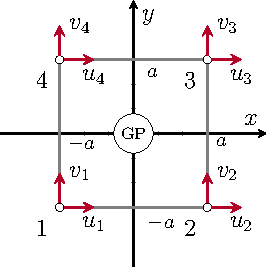
\includegraphics{figures/03_comparison_TO_TTO/03_gauss_point/gp.pdf}
    \caption{A four-node quadrilateral element. GP is the Gaussian integration point for which the equivalent stress is evaluated.}
    \label{fig:03_gp}
\end{marginfigure}


The stress tensor is evaluated using the elasticity Hooke's law in 2D as follows: 
\begin{equation}
    \begin{pmatrix}
    \sigma_x \\
    \sigma_y \\
    \tau_{xy}
    \end{pmatrix}
    =\matr{C}_e
    \begin{pmatrix}
    \varepsilon_\text{x} \\
    \varepsilon_\text{y} \\
    \gamma_{xy}
%     \end{pmatrix},
%     \quad
%    \text{with }
    \end{pmatrix}
    \quad
    \text{with}
    \quad
    \matr{C}_e = \frac{E}{1-\nu^2}
    \begin{pmatrix}
    1   &   \nu &   0   \\
    \nu &   1   &   0   \\
    0   &   0   &   G
    \end{pmatrix}.
\end{equation}

The equivalent Von Mises stress of the element can then be written as:
\begin{align}
    \langle \vect{\sigma}_{\text{VM}} \rangle &= \sqrt{\sigma_x^2 + \sigma_y^2 - \sigma_x \sigma_y+3\tau_{xy}} \\
    &= \sqrt{
    \begin{pmatrix}
    \sigma_x & \sigma_y & \tau_{xy}
    \end{pmatrix}
    \begin{pmatrix}
    1       &   -1/2    &   0   \\
    -1/2    &   1       &   0   \\
    0       &   0       &   3
    \end{pmatrix}
    \begin{pmatrix}
    \sigma_x \\
    \sigma_y \\
    \tau_{xy}
    \end{pmatrix}} \\
    &= \sqrt{\vect{q}_s^T\matr{B}_s^T\matr{C}_e^T\matr{D}_{\text{VM}}\matr{C}_e\matr{B}_s\vect{q}_s}
    \textrm{,  with } \matr{D}_{\text{VM}} = 
    \begin{pmatrix}
    1       &   -1/2    &   0   \\
    -1/2    &   1       &   0   \\
    0       &   0       &   3
    \end{pmatrix} \\
    \langle \vect{\sigma}_{\text{VM}} \rangle &= \sqrt{\vect{q}_s^T\matr{S}\vect{q}_s}, \quad
    \textrm{with } \matr{S} = \matr{B}_s^T\matr{C}_e^T\matr{D}_{\text{VM}}\matr{C}_e\matr{B}_s.
    \label{eq:03_VM_calc}
\end{align}
in which we used the notation introduced by Verbart~\sidecite{verbart_unified_2017} $\langle \dots \rangle$ to represent macroscopic (or homogenized) variables.
\paragraph{Microscopic and macroscopic stress}
In stress-constrained topology optimization, the element stress is usually evaluated using the microscopic stress formulation, assuming that there is no direct correlation between stress and density~\sidecite{duysinx_topology_1998}. Indeed, the use of the macroscopic stress in volume minimization optimization problems creates an all-void design~\sidecite{le_stress-based_2010}. The properties that the microscopic stress should present are:
\begin{enumerate}[label=(\roman*)]
    \item The stress criterion should be mathematically as simple as possible, as the relationship between Young's modulus and density. This permits a simple numerical implementation.
    \item To mimic the real physical behavior, the microscopic stress should be inversely proportional to density.
    \item The microscopic stress should converge to a non-zero value at zero density. This requisite is deduced from investigations into the asymptotic stress behavior in thin layers~\sidecite{verbart_unified_2017}.
\end{enumerate}

The relation between stress and displacement is written as:
\begin{equation}
    \langle \vect{\sigma}_{\text{VM}} \rangle = \matr{C}_e(\langle E \rangle) \langle \vect{\varepsilon} \rangle,
    \label{eq:03_stress_disp}
\end{equation}
where the variables between angular brackets $\langle \dots \rangle$ represent macroscopic variables. \marginnote{Equation~\eqrefnotext{eq:02_simp} reads as follows: $$ E_i(\rhophys_i) = E_{\textrm{min}} + \rhophys_i^p(E_0-E_{\textrm{min}}) $$ where the parameter $p$ is called SIMP penalization parameter, and it is used to reduce the quantity of intermediate densities, pushing the result to a black-and-white result.}

Combining (i) and (ii) with \eqsref{eq:02_simp} and \eqrefnotext{eq:03_stress_disp}, the microscopic stress can be written as:
\begin{equation}
    \vect{\sigma}_{\text{VM}} = \frac{\langle \vect{\sigma}_{\text{VM}} \rangle}{\rho^q_e} = \rho_e^{p-q} \matr{C}_e(E_0)\langle \vect{\varepsilon} \rangle,
\end{equation}
where the exponent $q$ is a number greater than 1.

One possible choice that satisfy all the requirements is $q=p$~\sidecite{le_stress-based_2010,verbart_unified_2017,holmberg_stress_2013,da_silva_stress-constrained_2019}. Thus, the microscopic stress is defined as:
\begin{equation}
    \vect{\sigma}_{\text{VM}} = \matr{C}_e(E_0)\langle \vect{\varepsilon} \rangle.
    \label{eq:03_micro_stress}
\end{equation}
The significance of microscopic stress becomes evident when considering an element with intermediate density, that is physically realized by a porous microstructure. The microscopic stress presented in \eqref{eq:03_micro_stress} measures the stress in the material of the microstructure. It is grounded in the assumption that the macroscopic deformations of the homogenized element generate within the microstructure of the element a stress state that remains unaffected by the density of the element itself.

\paragraph{Constraints aggregation and relaxation}
When optimizing a structure with stress constraints using a \gls{nand} formulation, two primary challenges commonly arise:
\begin{enumerate}[label=(\roman*)]
    \item Is it known in the literature \sidecite{rozvany_design-dependent_2001,stolpe_models_2003} that stress-based topology optimization suffers from the \textit{singular minima} (or \textit{singularity}) problem: firstly observed on truss structure optimization \sidecite{sved_structural_1968}, these \textit{minima} are almost inaccessible to a standard gradient-based optimizer, often preventing it to reach the global optimum of the optimization~\cite{rozvany_design-dependent_2001}. This is because achieving the optimal solution to a problem using continuous design variables may necessitate passing through a state where the optimization constraints are violated, \ie the \textit{minimum} is on a lower dimension compared to the design space. This problem is often solved using a technique called \textit{constraints relaxation}~\sidecite{cheng_relaxed_1997}.
    \item The stress is a local measure, and thus a large set of constraints is generated when a reasonably fine mesh is used (one element, one constraint). This problem is often solved using a technique called \textit{constraints aggregation} or \textit{global constraints}~\sidecite{da_silva_local_2021}.
\end{enumerate} 

Following the work developed by Verbart \etal~\sideciteonce{verbart_unified_2017}, the lower bound \gls{ks} function~\sidecite{kreisselmeier_systematic_1979} is used to approximate the local relaxed stress constraint maximum. The authors showed that employing lower-bound \gls{ks} aggregation functions to approximate the maximum operator in stress-constrained topology optimization ensures the relaxation and aggregation of the constraints simultaneously. The \marginnote{We remember that the stress constraints are defined as follows: $$ \bar{\vect{g}}:=\rhophys_i\left(\frac{ \sigma_{\text{VM},i}}{\sigma_\text{L}}-1 \right) \leq 0. $$}\gls{ks} aggregated stress constraint function is defined as follows:
\begin{equation} 
    G_{\text{KS}}^\text{L} = \frac{1}{P} \ln{\left( \frac{1}{N_\text{e}} \sum e^{{P}\bar{g}_i} \right)}.
    \label{eq:03_gksl}
\end{equation}
Its main advantage over other different formulations is that it uses a single hyperparameter $P$ to control the aggregation and the relaxation of the constraints simultaneously.

\paragraph{Minimum volume formulation}
The \gls{nand} minimum volume formulation for continuous discretization is written combining \eqsref{eq:03_obj_vol} and \eqrefnotext{eq:03_gksl} as:
\begin{equation}
    \begin{aligned}
    \min_{\bm{\rho}}         && V &= \frac{1}{N_{e}} \sum_{i \in \Omega} \rhophys_i, && \text{(Volume minimization)} \\
    \textrm{s.t.}   && G_{\text{KS}}^\text{L} &= \frac{1}{P} \ln{\left( \frac{1}{N_\text{e}} \sum_{i \in \Omega} e^{{P}\bar{g}_i} \right)} \leq 0 && \textrm{(Stress constraints)}\\
    && \bm{K}\bm{u} &= \bm{F} && \textrm{(FEM equation)}\\
    && 0 &\leq \rho_i \leq 1, \\
    \end{aligned}
    \tag{$\mathbb{T}_1$}
    \label{eq:03_prob-stress}
\end{equation}
The optimization is carried out using a gradient descent optimization algorithm for which the sensitivities are given in analytical form. Using analytic gradients is in general more efficient than finite differences as it avoids the need for multiple function evaluations, making the optimization process faster and more precise.

\paragraph{Sensitivity analysis of the objective function}
Deriving \eqref{eq:03_obj_vol} with respect to $\rhophys$ we obtain:
\begin{equation}
    \derfrac{V}{\rhophys_i} = \frac{1}{N_{e}}.
    \label{eq:03_01}
\end{equation}
The sensitivity of the objective function can then be evaluated using \eqref{eq:03_01} as follows:
\begin{equation}
    \frac{d V}{d \rho_i} = \sum_{j \in \mathbb{N}_{i,R}} \derfrac{V}{\rhophys_j} \derfrac{\rhophys_j}{\rhofil_j} \derfrac{\rhofil_j}{\rho_i}.
\end{equation}
in \marginnote{\eqref{eq:02_rhofil} reads: $$ \rhofil_i = \frac{\sum_{j \in \mathbb{N}_{i,R}} w(d_j)v_j\rho_j}{\sum_{j \in \mathbb{N}_{i,R}} w(d_j)v_j}.$$} which the derivative of the filtered density $\vect{\rhofil}$ with respect to the design variable $\vect{\rho}$ is written deriving \eqref{eq:02_rhofil}:
\begin{equation}
    \derfrac{\rhofil_i}{\rho_j} = \frac{w(d_j)v_j}{\sum_{j \in \mathbb{N}_{i,R}} w(d_j)v_j}.
    \label{eq:03_sens_filt}
\end{equation}
The \marginnote{\eqref{eq:02_proj} reads: $$ \rhophys_j = \frac{\tanh(\beta\eta)+\tanh(\beta(\rhofil_j - \eta))}{\tanh(\beta\eta)+\tanh(\beta(1 - \eta))}.$$} sensitivity of the physical densities $\bm{\rhophys}$ with respect to the filtered $\bm{\rhofil}$ can be written deriving \eqref{eq:02_proj} as:
\begin{equation}
    \derfrac{\rhophys_j}{\rhofil_j} = \beta \frac{1-\tanh^2(\beta(\rhofil_j-\eta))}{\tanh(\beta\eta)+\tanh(\beta(1 - \eta))}.
    \label{eq:03_sens_proj}
\end{equation}
Using the chain rule it is possible to write:
\begin{equation}
    \label{eq:03_chain}
    \derfrac{h}{\rho_i} = \sum_{j \in \mathbb{N}_{i,R}} \derfrac{h}{\rhophys_j} \derfrac{\rhophys_j}{\rhofil_j} \derfrac{\rhofil_j}{\rho_i},
\end{equation}
where $h$ represents a generic function.
\paragraph{Sensitivity analysis of the constraint function}
The sensitivity of the aggregated constraint function $G_{\text{KS}}^\text{L}$ with respect to the design variable $\vect{\rho}$ is evaluated using:
\begin{equation} \label{eq:03_chain_sens_fin}
    \frac{d G_{\text{KS}}^\text{L}}{d \rho_i} = \sum_{j \in \mathbb{N}_{i,R}} \derfrac{G_{\text{KS}}^\text{L}}{\rhophys_j} \derfrac{\rhophys_j}{\rhofil_j} \derfrac{\rhofil_j}{\rho_i}.
\end{equation}

As \marginnote{we remember that $$\matr{K}(\vect{\rhophys})\vect{u}=\vect{f}$$} the constraint function $G_{\text{KS}}^\text{L} = G(\vect{\rhophys}, \vect{u}(\vect{\rhophys}) )$ is explicitly and implicitly (via the relationship with $\vect{u}$) depending on $\vect{\rhophys}$, the first-order derivative is evaluated using the total derivative formula:
\begin{equation} \label{eq:03_sens-0}
    \frac{d G}{d \rhophys_j} = \derfrac{G}{ \rhophys_j} + \derfrac{G}{\vect{u}} \derfrac{\vect{u} }{\rhophys_j}.
\end{equation}
As function $G_{\text{KS}}^\text{L}$ depends on $\vect{u}$ via the stresses $\sigma_i$, it is possible to write:
\begin{equation} \label{eq:03_sens-1}
    \derfrac{G}{\vect{u}} = \sum_{i \in \Omega} \left( \derfrac{G}{\sigma_i} \derfrac{\sigma_i}{\vect{u}}\right).
\end{equation}
Combining Eq. \ref{eq:03_sens-0} with Eq. \ref{eq:03_sens-1}, we obtain:
\begin{equation} \label{eq:03_sens-2}
    \frac{d G}{d \rhophys_j} = \underbrace{\derfrac{G}{\rhophys_j}}_A + \sum_{i \in \Omega} \left( \underbrace{\derfrac{G}{\sigma_i}}_B \underbrace{\derfrac{\sigma_i}{\vect{u}}}_C \right)  \underbrace{\derfrac{\vect{u} }{\rhophys_j}}_D.
\end{equation}
We compute the four factors separately:
\begin{enumerate}[label=\Alph* --]
    \item The first term represents the explicit relationship of $G$ to the physical densities and its calculation is straightforward: 
    \begin{equation} \label{eq:03_sens-2-1}
        \derfrac{G}{ \rhophys_j} = \frac{1}{P} \frac{\left(\frac{ \sigma_{\text{VM},j}}{\sigma_\text{L}}-1 \right)\frac{1}{N_\text{e}} P e^{{P}\bar{g}_j}}{\frac{1}{N_\text{e}} \sum_k e^{{P}\bar{g}_k}} = \left(\frac{ \sigma_{\text{VM},j}}{\sigma_\text{L}}-1 \right) \frac{e^{{P}\bar{g}_j}}{\sum_k e^{{P}\bar{g}_k}}.
    \end{equation}
    
    \item The second term can be calculated using the chain rule:
    \begin{equation}
        \label{eq:03_sens-2-2}
        \derfrac{G}{\sigma_i} = \derfrac{G}{\bar{g}_i} \derfrac{\bar{g}_i}{\sigma_i} = \frac{1}{P} \frac{\frac{1}{N_\text{e}} P e^{{P}\bar{g}_i}}{\frac{1}{N_\text{e}} \sum_k e^{{P}\bar{g}_k}} \frac{\rhophys_i}{\sigma_\text{L}} = \frac{\rhophys_i}{\sigma_\text{L}} \frac{e^{{P}\bar{g}_i}}{\sum_k e^{{P}\bar{g}_k}}.
    \end{equation}
    
    \item We reformulate \eqref{eq:03_VM_calc} \marginnote{\eqref{eq:03_VM_calc} reads: $$ \langle \vect{\sigma}_{\text{VM}} \rangle = \sqrt{\vect{q}_s^T\matr{S}\vect{q}_s}.$$} to be written in global coordinates instead of local:
    \begin{equation}
        \label{eq:03_sens-3}
        \sigma_i^2 = \vect{q}_s^T\matr{S}\vect{q}_s = \vect{u}^T \matr{S}_g \vect{u},
    \end{equation}  
    where $\matr{S}_g$ represents the matrix $\matr{S}$ of \eqref{eq:03_VM_calc} written on global coordinates \sidenote{The matrix $\matr{S}_g$ can be calculated using the very same assembling approach used for the stiffness matrix $\matr{K}$ starting from the elemental stiffness matrix $\matr{K}_e$. As the global stiffness matrix $\matr{K}$, $\matr{S}_g$ is symmetric and sparse.}. We can now differentiate \eqref{eq:03_sens-3} with respect of the displacement field in global coordinates $\vect{u}$ to obtain:
    \begin{equation}
        \label{eq:03_sens-4}
        \derfrac{\sigma_i}{\vect{u}} = \frac{\matr{S}_g \vect{u}}{\sigma_i}.
    \end{equation}
    \eqsref{eq:03_sens-2-2} and \eqrefnotext{eq:03_sens-4} are now combined to obtain the result of the product of the \textbf{B} and \textbf{C} terms. As a result, the derivatives of $G$ with respect to $\bm{u}$, are written as:
    \begin{equation} \label{eq:03_sens-4-1}
        \derfrac{G}{\vect{u}} = \frac{\frac{\rhophys_j}{\sigma_\text{L}\sigma_j} e^{{P}\bar{g}_i}}{\sum_i e^{{P}\bar{g}_i}} |\bm{S_j}|_g \bm{u}.
    \end{equation}

    \item To calculate the last term, we take the static equilibrium equation $\matr{K}\vect{u} = \vect{f}$ and differentiate it with respect to the physical densities $\rhophys_j$, obtaining:
    \begin{equation}
        \derfrac{\matr{K}}{\rhophys_j}\vect{u} + \matr{K}\derfrac{\vect{u}}{\rhophys_j} = 0 \iff \derfrac{\vect{u}}{\rhophys_j} = -\matr{K}^{-1}\derfrac{\matr{K}}{\rhophys_j}\vect{u},
    \end{equation}
    where
    \begin{equation}
        \label{eq:03_sens-5}
        \derfrac{\matr{K}}{\rhophys_{j}} = (E_0-E_{\textrm{min}}) p\rhophys_j^{p-1} \matr{K}_{e,j}.
    \end{equation}
    \eqref{eq:03_sens-5} represent the well-known first-derivative term of the global stiffness matrix $\matr{K}$ with respect to the physical densities $\rhophys_j$ when using \gls{simp} material scheme~\sidecite{bendsoe_topology_2004}. We obtain the last term:
    \begin{equation} \label{eq:03_sens-6}
        \derfrac{\vect{u} }{\rhophys_j} = - \matr{K}^{-1} \left((E_0-E_{\textrm{min}}) p\rhophys_j^{p-1} \matr{K}_e \right) \vect{u}.
    \end{equation}
\end{enumerate}

Combining Eq. \ref{eq:03_sens-2}, Eq. \ref{eq:03_sens-2-1}, Eq. \ref{eq:03_sens-4-1}, and Eq. \ref{eq:03_sens-6}, we finally obtain:
\begin{equation}
\derfrac{G_{\text{KS}}^\text{L}}{\rhophys_j} = \left(\frac{ \sigma_{\text{VM},j}}{\sigma_\text{L}}-1 \right) \frac{e^{{P}\bar{g}_j}}{\sum_k e^{{P}\bar{g}_k}} - 
\matr{K}^{-1}\derfrac{G}{\vect{u}} \left(\derfrac{\matr{K}}{\rhophys_{j}} \right) \vect{u}.
\end{equation}

To avoid the explicit calculation of $\matr{K}^{-1}$ we use the \textit{adjoint method}\sidenote{More information about the adjoint method used to analytically calculate the first-order derivatives can be found on the Martins \etal book \cite{martins_engineering_2021}.}. Here is the linear system that, once solved, permits to calculate $\vect{\psi}$:
\begin{equation} \label{eq:03_sens-98}
    \matr{K}\vect{\psi} = \derfrac{G}{\vect{u}} \iff \vect{\psi} = \matr{K}^{-1}\derfrac{G}{\vect{u}}.
\end{equation}
This formula is called \textit{adjoint equation}. This equation is solved for $\vect{\psi}$ and the result used to evaluate:
\begin{equation}\label{eq:03_sens-99}
\derfrac{G_{\text{KS}}^\text{L}}{\rhophys_j} = \left(\frac{ \sigma_{\text{VM},j}}{\sigma_\text{L}}-1 \right) \frac{e^{{P}\bar{g}_j}}{\sum_k e^{{P}\bar{g}_k}} - \vect{\psi} \left(\derfrac{\matr{K}}{\rhophys_{j}}\right) \vect{u}.
\end{equation}
\marginnote{Solving linear system \ref{eq:03_sens-98} instead of directly calculating the inverse matrix of $\matr{K}$ is more efficient from a performance perspective. The cost of solving a system using the Cholesky decomposition is $\mathcal{O}(N^3/3)$, while a matrix inversion is $\mathcal{O}(N^3)$.} where $N$ represents the size of the square matrix describing the linear system.
\eqref{eq:03_sens-99} represents the first-order derivative equation used to evaluate the sensitivity of the constraint function $G_{\text{KS}}^\text{L}$ with respect to the physical densities $\vect{\rhophys}$. The value of $\vect{\psi}$ is calculated every iteration solving the linear system \ref{eq:03_sens-98}.

\subsection{\acrfull{tto} minimum volume formulation}
We are now shifting our focus from continuous structures to discrete truss systems, describing the \acrfull{tto} (also known in early literature as layout optimization), a structure optimization method that focuses on discrete structures. In his most used formulation, \gls{tto} aims at reducing structural volume while meeting stress criteria using a \gls{sand} approach. The problem is already well-posed for the comparison with continuous discretization.

\paragraph{Objective and constraint functions} 
The goal of the optimization is to minimize the volume occupied by a structure under a specified load case. For a truss structure, we can write:
\begin{equation}
    V = \vect{\ell}^{T}\vect{a}
\end{equation}
in which $\vect{\ell} = [\ell_1, \ell_2, \ldots,\ell_{N\text{el}}]^T$ is the length vector of the member of the ground structure. The volume fraction is evaluated as the ratio $ V_\text{f} = \frac{V}{V_0}$, where $V_0$ represents the total volume of the design domain $\Omega$.

As the volume minimization problem is stated using the \gls{sand} approach, both the members' cross-sectional areas $\vect{a}$ and member forces $\vect{q}$ are design variables of the problem. For that reason, the stress constraints in tension and compression ($\vect{g}_\text{st,t}$ and $\vect{g}_\text{st,c}$) can be trivially written as:
\begin{equation}
    -\sigma_\text{c}\vect{a} \leq \vect{q} \leq \sigma_\text{t}\vect{a}
\end{equation}
in which $\sigma_\text{c}$ and $\sigma_\text{t}$ are the compressive and tensile maximum allowable stresses of the material.

\paragraph{Minimum volume formulation}
We recall the full volume minimization formulation here, stated in terms of members' cross-sectional areas $\vect{a}$ and member forces $\vect{q}$ as follows:
\begin{equation}
    \begin{aligned}
    \min_{\vect{a}, \vect{q}}   && V &= \vect{\tilde{\ell}}^{T}\vect{a} && \textrm{(Volume minimization)}\\
    \textrm{s.t.}   && \matr{B}\vect{q} &= \vect{f} && (g_\text{eq})\\
    && -\sigma_\text{c}\vect{a} &\leq \vect{q} \leq \sigma_\text{t}\vect{a} && (g_\text{st,c}, \; g_\text{st,t}) \\
    && \vect{a} &\geq 0, \\
    \end{aligned}
    \tag{$\mathbb{P}_0$}
    \label{eq:03_optim_original}
\end{equation}
where $\vect{\tilde{\ell}} = [\ell_1 + s, \ell_2 + s, \ldots,\ell_{N\text{el}} + s]^T$ is called augmented member length and $s$ the joint cost, used to penalize the appearance of small members~\sidecite{parkes_joints_1975}. The listing and explanation of the other parameters is given in \secref{sec:02_tto}. This formulation takes into account only the linear behavior of the structure and is equivalent to the original and well-studied member force formulation~\sidecite{dorn_automatic_1964, bendsoe_topology_2004}. 

It is worth listing the key distinctions of the \gls{tto} formulation compared to the density-based topology optimization formulation described earlier in this chapter. Firstly, the \gls{tto} problem is formulated using the \gls{sand} approach, in which the equations of structural mechanics are treated as constraints in the optimization. Unlike \gls{nand} approaches, these equations are not explicitly solved. Consequently, concerns about the singularity of the stiffness matrix $\matr{K}$ are avoided, and bars can potentially vanish from the structure during the optimization ($a=0$). Secondly, the \gls{tto} problem is expressed in terms of members' cross-sectional areas $\vect{a}$ and member forces $\vect{q}$ with a plastic material model, disregarding kinematic compatibility to formulate a \gls{lp} problem. Due to its linearity, this optimization problem is convex, ensuring that the solutions found are global optima. Moreover, the linear nature of the formulation \ref{eq:03_optim_original} makes it computationally efficient, even with a large number of design variables, when employing modern interior point optimizers. However, the \gls{sand} formulation with a plastic material model accurately predicts the mechanical behavior of only statically determinate structures or mechanisms~\sidecite{kirsch_optimal_1989, rozvany_layout_1995}. When dealing with more complex structures, such as those that are statically indeterminate due to symmetry or multiple load cases, explicit consideration of the linear kinematic constraints is necessary, leading to a loss of the linear property of the formulation.

\section{Comparison between density-based topology optimization and TTO} \label{sec:03_comparison}
In the upcoming discussion, we will be comparing the optimized structures obtained using the density-based topology optimization and the \gls{tto} optimization algorithms. Our primary objective in this comparison is to choose the most appropriate method for our study by understanding the application limits inherent in these two structural discretization methods. If, indeed, we identify such limitations, the aim is to discern and define them. Such discussions have already been briefly addressed in the literature~\sidecite{bendsoe_optimal_1989, watts_simple_2019}, but treating the problem without providing numerical results as a basis for making the choice.

Since our interest is in ultralight structures, we are willing to compare the results of both optimization methods when dealing with different volume fractions on a common load case. The volume minimization formulation with stress constraints we use cannot, however, directly control the volume of the optimized structure. For that reason, we decided to adjust the material strength $\sigma_\text{L}$ to influence the volume fraction of the optimized structure \ie employing more resistant material results in a lower volume fraction and \textit{vice versa}. For this comparative analysis, we have selected three key performance metrics: the volume fraction $V_\text{f}$, the structural compliance $C$, and the maximum material allowable -- or strength $\sigma_\text{L}$. Among these, we classify stress limit as the active metric used to influence the optimization, while volume and compliance are the objective of the optimization and a passive metric, respectively. In addition to the aforementioned performance metrics, we will also track the execution time of the algorithms.

\subsection{Definition of a test case for the comparison}
\begin{figure}
    \centering
    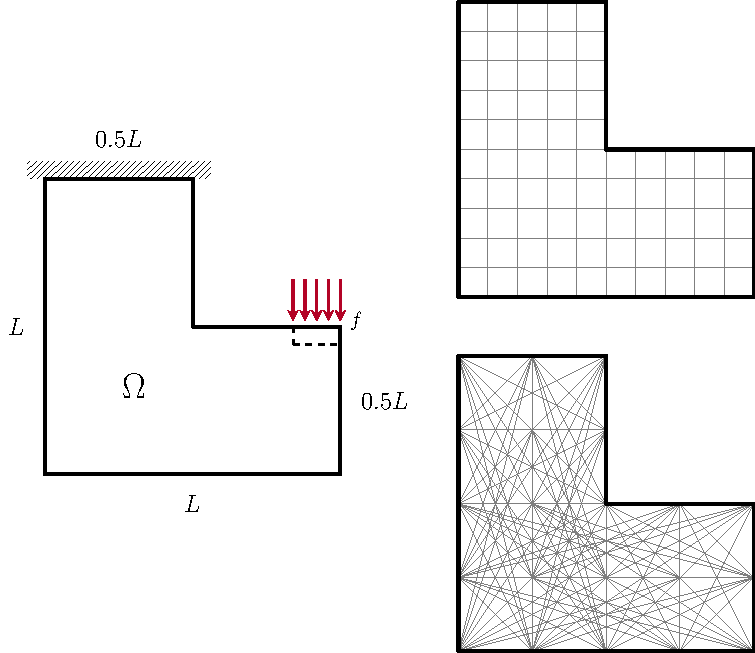
\includegraphics[scale=0.75]{figures/03_comparison_TO_TTO/06_L_bc/L_bc.pdf}
    \caption{On the left, plot of the L-shape beam test case, on the right the graphical representations of the two discretizations used, the continuous (above) composed of $600\times600$ quadrilateral elements, and the truss-like (below) discretized using $33\times 33$ nodes and a fully connected ground structure. The images represent a coarser discretization for visual clarity.}
    \label{fig:03_L_bc}
\end{figure}
The L-shape beam is one of the most used load case benchmarks for stress-based topology optimization~\sidecite{duysinx_topology_1998,le_stress-based_2010}. This choice is driven by the distinctive geometry of the problem, which generates a stress concentration at the sharp corner in the case of linear elasticity—a phenomenon approaching infinity. Consequently, optimized solutions often feature a large fillet, mitigating the intensity of the stress singularity. The geometric description of the test case is given in \figref{fig:03_L_bc}. The beam with dimensions $L\times L$ presents a fixed support on the nodes in the top part and a load on the right extremity.

To permit the methods' comparison, the design domain $\Omega$ is discretized using two distinct meshes: in the continuous case, we employ a mesh consisting of $600\times600$ quadrilateral elements, totaling \num[group-separator={$\,$}]{270000} elements. For this mesh, the load is distributed over multiple elements (5\% of $L$) to avoid local stress concentrations. Additionally, the stress constraints are not evaluated on the corresponding elements, and this zone is considered outside of the design domain $\Omega$. Concerning the truss discretization for the \gls{tto} algorithm, we employ a mesh with $33\times 33$ nodes and a fully connected ground structure, comprising a total of \num[group-separator={$\,$}]{305728} candidates. The load is applied only on one single node.

We employ the same isotropic material and structure dimensions for the two optimizations, and the complete data is resumed in \tabref{tab:03_mat}. The value of the maximum material allowable $\sigma_\text{L}$ is used to control, although not directly, the volume fraction of the solutions. For simplicity, all numeric values are assumed normalized and dimensionless.

\begin{margintable}
    \small
    \centering
    \begin{tabular}{cc}
    \toprule
    \textbf{Parameter}        & \textbf{Value} \\ \midrule
    $E$              & 1     \\
    $\nu$            & 0.3   \\
    $L$              & 100   \\
    $\sigma_\text{L}$ & $[0.20,20]$ \\
    \bottomrule
    \end{tabular}
    \caption{Material data used for the optimizations. The value of the maximum material allowable $\sigma_\text{L}$ is used as the parameter to generate multiple optimized topologies. The Poisson module is used only in density-based topology optimization.}
    \label{tab:03_mat}
\end{margintable}

\subsection{Numerical application} \label{sec:03_applications}
The density-based topology optimization and the \gls{tto} have both been implemented using Python, employing different optimization algorithms. For density-based topology optimization, the chosen optimization algorithm is the \gls{mma}, developed by Svanberg~\sidecite{svanberg_method_1987}. The parameter called \textit{movelimit}\sidenote{More information on the implementation of the \textit{movelimit} parameter can be found on the paper by Verbart \cite{verbart_unified_2017}.} is set to $0.1$ while the other algorithm's parameters are set to their default value. We chose to filter the density field $\vect{\rho}$ using the 2D convolution operator~\sidecite{sigmund_morphology-based_2007} and the projection technique based on the \textit{tanh} function~\sidecite{wang_projection_2011} precedently described. The radius of the filter is set to $R=5$ elements. \marginnote{\eqref{eq:02_proj} reads: $$  \rhophys_j = \frac{\tanh(\beta\eta)+\tanh(\beta(\rhofil_j - \eta))}{\tanh(\beta\eta)+\tanh(\beta(1 - \eta))}. $$} Using the projection \eqref{eq:02_proj} is not volume conservative for all values of $\eta$, and to stay conservative we use a volume-increasing filter~\sidecite{ferrari_new_2020}. The value of $\eta = 0.4$ is then chosen. A continuation scheme for the projection parameter $\beta$ is set to increase by one every 200 iterations and starting from 1, the number of maximum iterations is set to 7500, and the stopping criteria is calculated as $\Vert \Delta \vect{x} \Vert_2 / \sqrt{N_\text{e}}$ \cite{ferrari_new_2020} on the absolute difference between two successive iterations of the physical densities $\rhophys$, and it is set to $10^{-4}$. The aggregation parameter $P$ of the aggregation function $G_{\text{KS}}^\text{L}$ is set to 32. The \gls{simp} parameters of \eqref{eq:02_simp} are set to $E_0 = 1$, and $E_{\textrm{min}} = 10^{-9}$. The value of the penalization parameter $p$ is selected as $p=3$. The optimization is carried out using the NLopt Python optimization package~\sidecite{NLopt_2007}, analytically evaluating the sensitivity using \eqsref{eq:03_01} and \eqrefnotext{eq:03_sens-2}.

The volume minimization \gls{tto} problem as formulated in \ref{eq:03_optim_original} represents a \gls{lp} problem that can be efficiently solved by contemporary optimization algorithms. In this work, we used the Python package CVXPY 1.2.2~\sidecite{diamond_cvxpy_2016} with the ECOS 2.0.7~\sidecite{domahidi_ecos_2013} solver. The joint cost $s$ is set to 0.001 and the stopping criterion is chosen as $\norm{\Delta \vect{x}}_\infty \leq 10^{-8}$. As the formulation is linear, no sensitivity calculation is carried out.

The optimizations presented in this section are performed using a single core on a cluster equipped with an Intel® Xeon® CPU E5-2650 @ \qty{2.20}{GHz} and using \qty{8}{GB} of RAM.

\paragraph{density-based topology optimization results}
\begin{figure*}
    \subcaptionbox{}{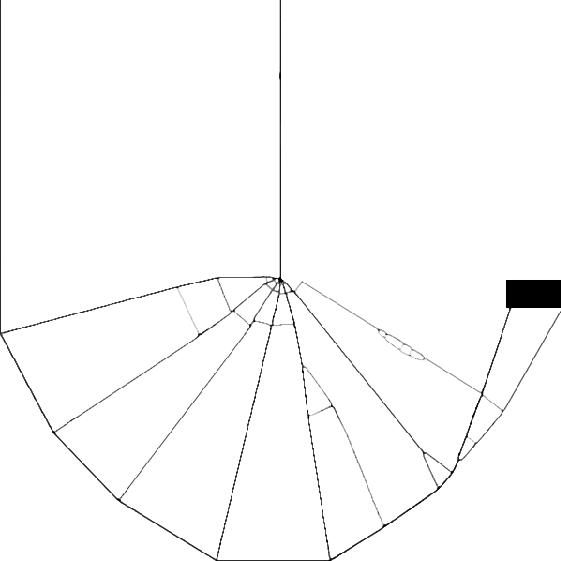
\includegraphics[width=0.23\linewidth ]{figures/03_comparison_TO_TTO/07_to_sol/fig0_10.pdf}}
    \hfill
    \subcaptionbox{}{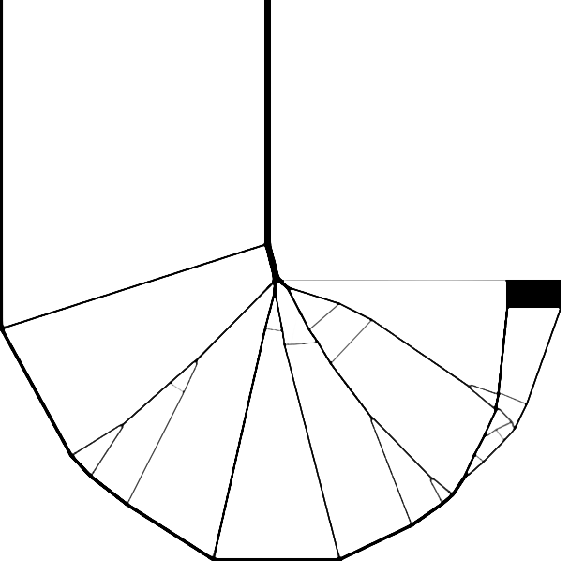
\includegraphics[width=0.23\linewidth ]{figures/03_comparison_TO_TTO/07_to_sol/fig0_2.pdf}}
    \hfill
    \subcaptionbox{}{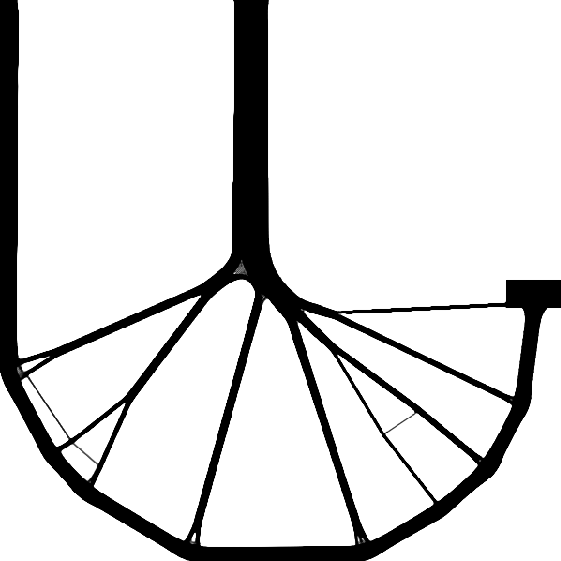
\includegraphics[width=0.23\linewidth ]{figures/03_comparison_TO_TTO/07_to_sol/fig0_0.4.pdf}}
    \hfill
    \subcaptionbox{}{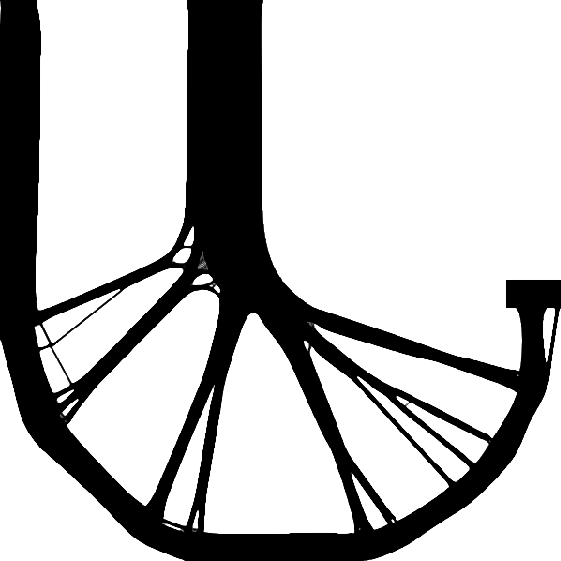
\includegraphics[width=0.23\linewidth ]{figures/03_comparison_TO_TTO/07_to_sol/fig0_0.25.pdf}}
    \bigskip
    \subcaptionbox{}{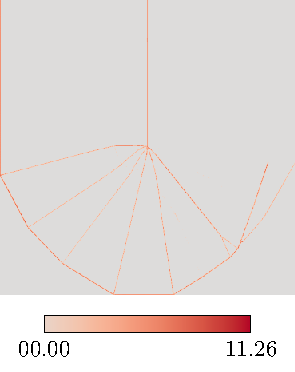
\includegraphics[width=0.23\linewidth ]{figures/03_comparison_TO_TTO/07_to_sol/stress_10.pdf}}
    \hfill
    \subcaptionbox{}{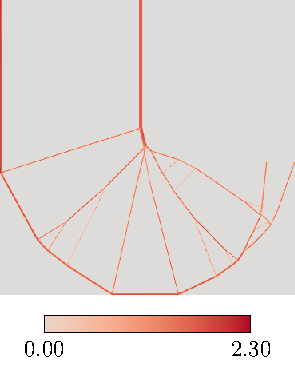
\includegraphics[width=0.23\linewidth ]{figures/03_comparison_TO_TTO/07_to_sol/stress_2.pdf}}
    \hfill
    \subcaptionbox{}{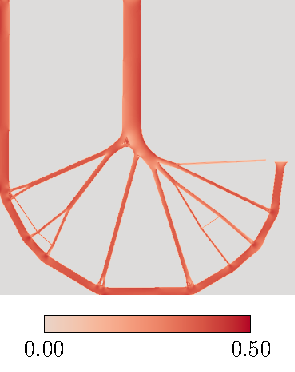
\includegraphics[width=0.23\linewidth ]{figures/03_comparison_TO_TTO/07_to_sol/stress_04.pdf}}
    \hfill
    \subcaptionbox{}{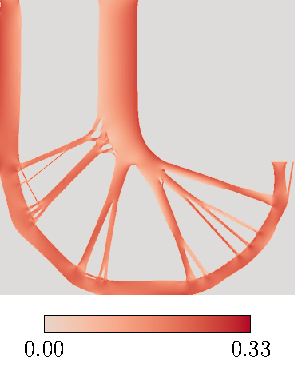
\includegraphics[width=0.23\linewidth ]{figures/03_comparison_TO_TTO/07_to_sol/stress_025.pdf}}
    \caption{(a-d) Topology of the optimized structures for different values of the material allowable $\sigma_\text{L}=10.00$, 2.00, 0.40, and 0.25, showing a volume fraction of $V_\text{f}=1.60\%$, $4.04\%$, $18.03\%$ and $34.71\%$, respectively. (e-h) Von Mises stress distribution for the optimized structures.}
    \label{fig:03_to_sol}
\end{figure*}
We generate multiple optimized structures with different volume fractions $V_\text{f}$ by launching the optimization code for continuous mesh with different values of the material allowable $\sigma_\text{L}$ spanning from $0.2$ to $20$.

The results obtained for $\sigma_\text{L}=10.00,2.00,0.40\text{ and }0.25$ are shown in \figref{fig:03_to_sol}. In the upper part of the figure (a-d), we see the topology of the optimized structures with an increasing volume fraction $V_\text{f}$. Interestingly, the topology of the solution remains almost unchanged, varying principally in the thickness of its members. We notice the classic large fillet around the corner that alleviates the local stress concentration. As the volume decreases, the optimized structure tends to a solution that resembles a truss-like structure, with a reducing fillet radius. In those cases, we know that the density-based topology optimization algorithm acts as a method for the layout of truss-like structures~\sidecite{bendsoe_generating_1988}. This effect is caused by the combination of different factors, such as the regularization filter, the mesh size, and the low volume fraction~\sidecite{sigmund_non-optimality_2016}. 

A summary of the numerical results is presented in \tabref{tab:03_TO_results}. Firstly, we can observe how we successfully controlled the volume fraction $V_\text{f}$ by modifying the material resistance $\sigma_\text{L}$, obtaining results that perfectly follow a monotonically decreasing function. Additionally, as expected, a more voluminous solution also exhibits a lower value of structural compliance. Next, we notice that the optimization processes exhibit long execution times, especially when dealing with extreme cases like low-material resistance and high-volume fractions. This effect is caused by the very fine mesh used to discretize the design domain $\Omega$, the sensitivity calculation using the adjoint method, and the increasing difficulty of satisfying the stress constraints. Furthermore, it is observed that the maximum stress exceeds the material allowable $\sigma_\text{L}$. This is because we are employing an aggregation function for the stress constraints that estimates the maximum value of the constraint across a group of elements. However, these aggregation methods do not perfectly align with the exact maximum value, which is a recognized limitation.

On top of volume fraction, compliance, and stress, we evaluate an additional metric specific to continuous meshes called the \textit{greyness level} or \textit{measure of non-discreteness}~\sidecite{sigmund_morphology-based_2007} to evaluate the quality of the solutions. It is defined as:
\begin{equation}
    M_\text{nd} = \frac{\sum_e 4 \rhophys_e(1-\rhophys_e)}{n} \times 100 \%,
\end{equation}
where results near zero mean a completely black-and-white design. Observing the $M_\text{nd}$ values in \tabref{tab:03_TO_results}, we notice that all the optimized structures converged to nearly black-and-white solutions, confirming the correct numerical implementation of the problem.

In the lower part of \figref{fig:03_to_sol} (e-f), we plot the equivalent Von Mises stress for every element of the solution with physical density $\rhophys>0.5$. Multiple interesting observations can be made. First, we notice that the stress distribution is almost uniform in the structure, and it tends to the value of the material allowable $\sigma_\text{L}$ -- \ie we approach a \textit{fully stressed} structure. Even if the geometric support of the theory is different, it looks like the topology-optimized structures follow the Michell criteria presented in \secref{sec:02_michell}\marginnote{Michell theorized two criteria for optimal truss structures~\cite{michell_limits_1904} valid when the maximum allowable stress is equal in tension and compression ($\sigma_\text{t} = \sigma_\text{c}$) and when the supports of the structure are statically determinate. The first one states that all the members of an optimal structure should present internal stress equal in magnitude to the maximum allowable value of the material -- \ie the structure is \textit{fully stressed}. The second criterion asserts that the strain of all the members of the structure should be equal and there should be no other point having a strain higher than this value.} for optimal truss structures. 

\begin{table}
    \small
    \centering
    \sisetup{table-auto-round}
    \begin{tabular}{S[table-format = 2.2]
                    S[table-format = 2.2]
                    S[table-format = 2.2]
                    S[table-format = 5.0]
                    S[table-format = 1.2]
                    S[table-format = 4.0]
                    c
                    }
    \toprule
    $\bm \sigma_\text{L}$ & $\bm \max \bm \sigma_\text{L}$   & $\bm V_\text{f}$     & $\bm C$ & $M_\text{nd}$  & {\textbf{It.}}  & {\textbf{Time}}      \\ \midrule
    20    & 23.51 & 1.18\ppercent       & 6992.10    & \qty{1.91}{\percent} & 1142     & $\hms{08;11;00}$ \\
    10    & 11.26 & 1.60\ppercent       & 3837.08    & \qty{2.19}{\percent} & 1147     & $\hms{07;55;00}$ \\
    8     & 8.78  & 1.74\ppercent       & 2765.60    & \qty{1.95}{\percent} & 792      & $\hms{05;39;00}$ \\
    6     & 7.15  & 1.89\ppercent       & 2243.31    & \qty{1.81}{\percent} & 806      & $\hms{05;35;00}$ \\
    5     & 5.81  & 2.17\ppercent       & 1823.12    & \qty{1.81}{\percent} & 849      & $\hms{05;53;00}$ \\
    4     & 4.69  & 2.67\ppercent       & 1423.54    & \qty{2.02}{\percent} & 894      & $\hms{06;12;00}$ \\
    3     & 3.47  & 3.00\ppercent       & 1132.79    & \qty{1.64}{\percent} & 993      & $\hms{06;45;00}$ \\
    2     & 2.30  & 4.04\ppercent       & 781.48     & \qty{1.45}{\percent} & 1189     & $\hms{08;20;00}$ \\
    1     & 1.18  & 7.28\ppercent       & 403.53     & \qty{1.35}{\percent} & 1621     & $\hms{11;41;00}$ \\
    0.90  & 1.06  & 8.09\ppercent       & 364.80     & \qty{1.31}{\percent} & 1656     & $\hms{11;36;00}$ \\
    0.80  & 0.96  & 8.82\ppercent       & 331.95     & \qty{1.21}{\percent} & 1937     & $\hms{15;21;00}$ \\
    0.70  & 0.84  & 10.05 \ppercent    & 291.89     & \qty{1.09}{\percent} & 1827     & $\hms{13;21;00}$ \\
    0.60  & 0.73  & 11.80 \ppercent    & 250.23     & \qty{1.19}{\percent} & 1955     & $\hms{14;21;00}$ \\
    0.50  & 0.61  & 14.18 \ppercent    & 213.01     & \qty{1.06}{\percent} & 2032     & $\hms{15;39;00}$ \\
    0.40  & 0.50   & 18.03\ppercent     & 169.90     & \qty{1.08}{\percent} & 2259     & $\hms{17;06;00}$ \\
    0.35  & 0.44  & 21.12 \ppercent    & 148.13     & \qty{1.15}{\percent} & 2421     & $\hms{19;29;00}$ \\
    0.30  & 0.38  & 26.21 \ppercent    & 125.69     & \qty{1.50}{\percent} & 3100     & $\hms{24;46;00}$ \\
    0.25  & 0.33  & 34.71 \ppercent    & 104.30     & \qty{1.04}{\percent} & 3484     & $\hms{27;39;00}$ \\
    0.20  & 0.27  & 48.08 \ppercent    & 76.56      & \qty{1.26}{\percent} & \color{accent_r_1}7500     & $\hms{91;46;00}$ \\ \bottomrule
    \end{tabular}
    \caption{Numerical results of the topology optimization method of the L-shape beam load case with varying material allowable $\sigma_\text{L}$ on a $600 \times 600$ elements mesh. Numbers in red highlight the results that have not converged.}
    \label{tab:03_TO_results}
    \end{table}
    
\begin{marginfigure}
        \centering
        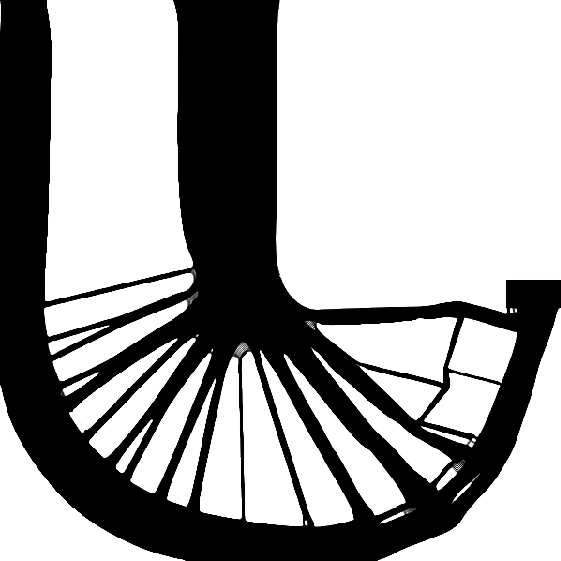
\includegraphics[width=0.8\linewidth]{figures/03_comparison_TO_TTO/08_to_no/fig0.pdf}
        \caption{The intermediate resulting structure for $\sigma_\text{L}=0.2$ with $V_\text{f}=\qty{48.08}{\percent}$ after 7500 optimization iterations.}
        \label{fig:03_to_sol_no}
    \end{marginfigure}

As previously mentioned, our focus lies in exploring the method's limits, particularly at the volume fraction boundaries. When dealing with low-resistance materials -- \ie materials that show a low $\sigma_\text{L}$, we encounter a scenario where no solution can be attained since no distribution can fulfill the imposed constraints. Throughout our research with this specific test case and mesh size, we did not produce any solutions with a volume fraction exceeding 50\%, suggesting we have encountered a limitation of the problem. With this combination of material properties, loading conditions, geometry, and mesh, it appears that there is no feasible solution for $V_\text{f} > 50\%$. We notice that the calculation time has significantly increased with the increase of $V_\text{f}$ because the algorithm needs more iterations to converge and faces greater difficulty in satisfying the stress constraints. \figref{fig:03_to_sol_no} shows the topology of the non-converged solution with $\sigma_\text{L}=0.2, \; V_\text{f}=\qty{48.08}{\percent}$ and over five days of optimization.
\begin{marginfigure}
    \centering
    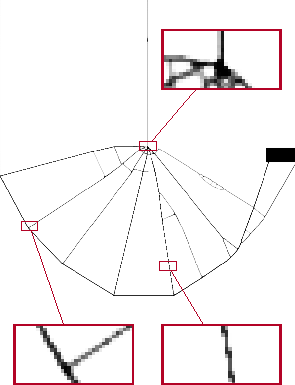
\includegraphics[width=0.8\linewidth]{figures/03_comparison_TO_TTO/09_to_zoom/to_zoom.pdf}
    \caption{The optimized structure for $\sigma_\text{L}=10.0$ with $V_\text{f}=\qty{1.60}{\percent}$. Some of the structure's features present not even a fully-dense element in their thickness.}
    \label{fig:03_to_sol_zoom}
\end{marginfigure}

Conversely, when dealing with excessively strong material -- \ie materials that show a high $\sigma_\text{L}$, the optimal scenario would demand such minimal material usage that certain sections of the structure become thinner than the width of a single element. In this case, the mesh used for discretization is too coarse to accurately represent the solution, and finer meshing becomes essential to capture the details of the optimized design. \figref{fig:03_to_sol_zoom} shows
the limit case when $\sigma_\text{L}=10.0$ and $V_\text{f}=\qty{1.60}{\percent}$.

Finally, in \figref{fig:03_to_plot} we show the plots summarizing our results, with the method's limits highlighted. To effectively show the different orders of magnitude present in the plot, we have used both linear and logarithmic scales simultaneously.
\begin{figure*}
    \hspace*{\fill}
    \subcaptionbox{\label{fig:03_to_plot_lin}}{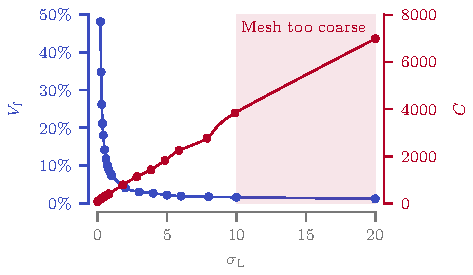
\includegraphics{figures/03_comparison_TO_TTO/10a_to_graph_lin/to_c_lin.pdf}}
    \hfill
    \subcaptionbox{\label{fig:03_to_plot_log}}{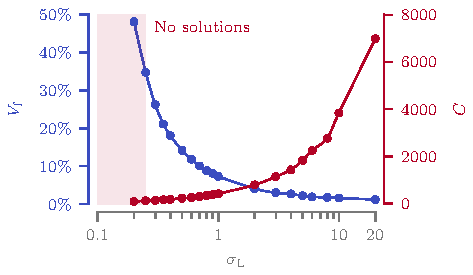
\includegraphics{figures/03_comparison_TO_TTO/10b_to_graph_log/to_c.pdf}}
    \hspace*{\fill}
    \caption{Linear (a) and logarithmic (b) plot of the volume fraction $V_\text{f}$ and the compliance $C$ with respect to the maximum material allowable $\sigma_\text{L}$ for the continuous mesh structures. Areas in red represent the zones outside the domains of applicability of the applied method.}
    \label{fig:03_to_plot}
\end{figure*}
We notice that the volume fraction $V_\text{f}$ follows a hyperbolic relationship, while compliance $C$ exhibits a linear correlation with respect to the material allowable $\sigma_\text{L}$.

\paragraph{TTO optimization results}
In this section, we present the optimized structures of the \gls{tto} formulation with different values of the material allowable $\sigma_\text{L}$ spanning from $0.2$ to $20$. Due to the inherent linearity of Formulation \ref{eq:03_optim_original}, the solutions exhibit several intriguing characteristics. Notably, in cases such as the tested L-shaped test case where the structures are not overconstrained and are not subject to asymmetric stress constraints, the formulation aligns with the Michell criteria. Consequently, the topology remains unchanged regardless of the imposed stress limit, and the stress distribution results in a fully stressed structure. \figref{fig:03_L_tto} provides a visual representation of the optimized topology and the corresponding stress distribution for the different values of the material allowable $\sigma_\text{L}$. By examining the figure, it is evident that the node positions are constrained by the initial ground structure. The solution resembles half of a spoked wheel, with an irregular distribution of these spokes. One might expect a more evenly distributed arrangement of these spokes. Interestingly, no fillet is formed at the corner of the L-shaped beam. This observation is attributed to the modeling of truss nodes as frictionless joints that do not support moments. However, this aligns with our earlier findings in density-based topology optimization, where the fillet radius diminishes as the volume fraction decreases. Finally, it is crucial to note that in this simple test case with only a single load case, linear elasticity is inherently considered in the formulation. There is no need to explicitly account for it by imposing kinematic compatibility constraints, as highlighted in previous studies \sidecite{dorn_automatic_1964,hemp_optimum_1973,bendsoe_topology_2004}.
\begin{figure}
    \centering
    \hspace*{\fill}
    \subcaptionbox{\label{fig:03_tto_sol_tc}}{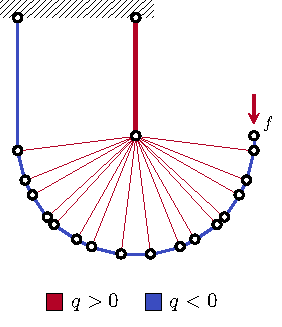
\includegraphics{figures/03_comparison_TO_TTO/11_tto_sol/L_tto_opt.pdf}}
    \hfill
    \subcaptionbox{\label{fig:03_tto_sol_st}}{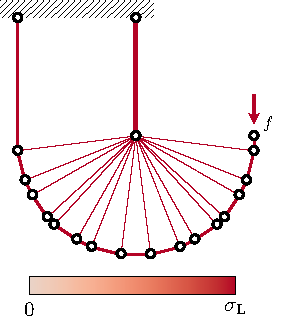
\includegraphics{figures/03_comparison_TO_TTO/11_tto_sol/L_tto_opt_st.pdf}}
    \hspace*{\fill}
    \caption{Topology (a) and stress distribution (b) plot for the \gls{tto} optimized structure of the L-shape beam test case with varying values of the material allowable $\sigma_\text{L}$ on a $33 \times 33$ nodes ground structure. The structure topology is invariant with respect to the value of $\sigma_\text{L}$.}
    \label{fig:03_L_tto}
\end{figure}

The following equation consistently holds for the optimized structures, regardless of the value of $\sigma_\text{L}$:
\begin{equation} \label{eq:03_V_star}
    V^*=\frac{fL}{\sigma_\text{L}}\cdot \Gamma,
\end{equation}
where the volume multiplicative constant $\Gamma$ depends on the load case and the ground structure used to discretize the design space $\Omega$ \sidecite{lewinski_extended_1994}. For this specific test case with the $33 \times 33$ nodes ground structure, we found $\Gamma=4.656$. The execution time of the optimization is approximately \qty{90}{\second} and does not change with respect to the maximum stress $\sigma_\text{L}$. The full numerical results of the multiple optimizations can be found in \tabref{tab:03_TTO_results}.

\begin{table}
    \small
    \centering
    \sisetup{table-auto-round}
    \begin{tabular}{S[table-format = 2.1]
                    S[table-format = 2.2]
                    S[table-format = 5.0]
                    S[table-format = 2.1]                    
                    S[table-format = 2.0]}
        
    \toprule
    $\bm \sigma_\text{L}$ & $\bm V_\text{f}$     & $\bm C$      & {\textbf{Min} $\bm \lambda$} & {\textbf{Time}} \\ \midrule
    50         & 0.124169\ppercent  & 23281.62 & 111.687                     & $\hms{00;01;06}$    \\
    20         & 0.310422\ppercent  & 9312.65  & 70.637                      & $\hms{00;01;09}$    \\
    10         & 0.620843\ppercent  & 4656.32  & 49.948                      & $\hms{00;01;18}$    \\
    8          & 0.776054\ppercent  & 3725.06  & 44.675                      & $\hms{00;01;15}$    \\
    6          & 1.034739\ppercent  & 2793.79  & 38.689                      & $\hms{00;01;10}$    \\
    5          & 1.241686\ppercent  & 2328.16  & 35.318                      & $\hms{00;01;24}$    \\
    4          & 1.552108\ppercent  & 1862.53  & 31.590                      & $\hms{00;01;18}$    \\
    3          & 2.069477\ppercent  & 1396.90  & 27.358                      & $\hms{00;01;15}$    \\
    2          & 3.104216\ppercent  & 931.26   & 22.337                      & $\hms{00;01;15}$    \\
    1          & 6.208431\ppercent  & 465.63   & 15.795                      & $\hms{00;01;17}$    \\
    0.90       & 6.898257\ppercent  & 419.07   & 14.984                      & $\hms{00;01;20}$    \\
    0.80       & 7.760539\ppercent  & 372.51   & \color{accent_r_1}14.127    & $\hms{00;01;21}$    \\
    0.70       & 8.869187\ppercent  & 325.94   & \color{accent_r_1}13.215    & $\hms{00;01;16}$    \\
    0.60       & 10.347385\ppercent & 279.38   & \color{accent_r_1}12.235    & $\hms{00;01;20}$    \\
    0.50       & 12.416862\ppercent  & 232.82  & \color{accent_r_1}11.169    & $\hms{00;01;22}$    \\
    \bottomrule    
    \end{tabular}
    \caption{Numerical results of the \gls{tto} method of the L-shape beam test case with varying values of the material allowable $\sigma_\text{L}$ on a $33 \times 33$ nodes ground structure. Numbers in red highlight the results that lie outside the domains of applicability of the optimization method.}
    \label{tab:03_TTO_results}
    \end{table}

    \begin{marginfigure}
        \centering
        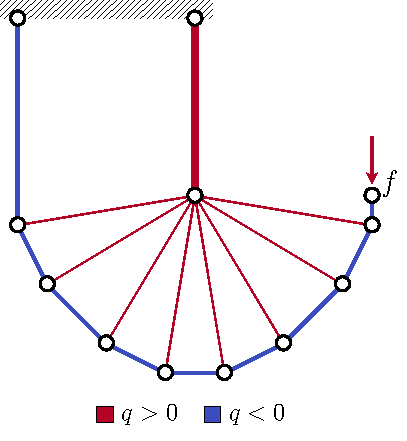
\includegraphics[width=0.8\linewidth]{figures/03_comparison_TO_TTO/12_tto_sol_13/L_tto_opt.pdf}
        \caption{Optimized structure obtained using a fully connected ground structure with $13 \times 13$ nodes and \num[group-separator={$\,$}]{7705} candidates.}
        \label{fig:03_L_tto_13}
    \end{marginfigure}
It's worth noting that we have intentionally opted for a dense ground structure here to achieve an element count roughly equivalent to that of the continuous mesh case (\num[group-separator={$\,$}]{305728} and \num[group-separator={$\,$}]{270000} for the \gls{tto} and the density-based topology optimization, respectively). We have utilized a fully connected ground structure with $33 \times 33$ nodes, but we obtained satisfactory results with just $13 \times 13$ nodes (see \figref{fig:03_L_tto_13}). In this case, we obtain a volume multiplicative constant $\Gamma=4.705$, signifying a \qty{1.05}{\percent} increase compared to the $33 \times 33$ case with $\Gamma=4.656$. However, the element number is reduced by \qty{97.4}{\percent} (\num[group-separator={$\,$}]{305728} versus \num[group-separator={$\,$}]{7705} candidates). The computational time for this simplified test case is below one second.

With this example, we notice that refining the continuous mesh and refining the ground structure are not equivalent operations. In one case, it allows for representing finer details, while in the other, it permits new shapes for the structure. The choice of the ground structure dictates the final form; it is more restrictive than merely allowing finer details. If bars are missing initially, they will not be added later on.

In assessing solution quality, we employ a distinct metric known as the slenderness ratio, denoted as $\lambda$, which represents the ratio between the length and the radius of gyration of the bars of the ground structure. In our specific case, we have established a minimum slenderness ratio of 15. For a bar with a circular cross-sectional area, this corresponds to a radius of $R_\lambda$ for a bar length of $7.5\;R_\lambda$. We highlighted in red the optimized structures that do not respect the minimum slenderness ratio in \tabref{tab:03_TTO_results}. 

Lastly, \figref{fig:03_tto_plot} provides a visual summary of our findings, emphasizing in red the solutions that do not respect the minimum slenderness ratio $\lambda<15$. To effectively show the different orders of magnitude present in the plot and how already done for the continuous mesh case, we have used both linear and logarithmic scales simultaneously. In this case, the compliance exhibits a perfectly linear relationship with respect to $\sigma_\text{L}$, while the volume follows a hyperbolic law in accordance with \eqref{eq:03_V_star}.

\begin{figure*}
    \hspace*{\fill}
    \subcaptionbox{\label{fig:03_tto_plot_lin}}{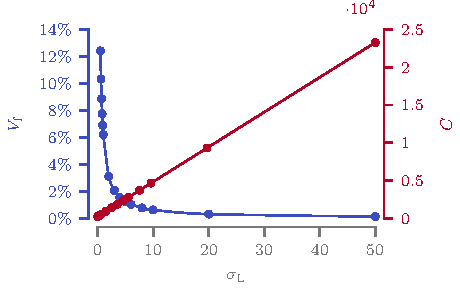
\includegraphics{figures/03_comparison_TO_TTO/13a_tto_graph_lin/tto_c_lin.pdf}}
    \hfill
    \subcaptionbox{\label{fig:03_tto_plot_log}}{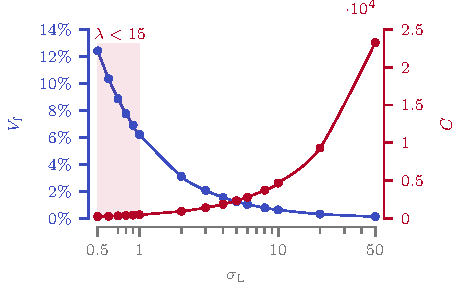
\includegraphics{figures/03_comparison_TO_TTO/13b_tto_graph_log/tto_c.pdf}}
    \hspace*{\fill}
    \caption{Linear (a) and logarithmic (b) plot of the volume fraction $V_\text{f}$ and the compliance $C$ with respect to the value of the maximum material allowable $\sigma_\text{L}$ for the \gls{tto} optimized structures. Areas in red represent the zones outside the domains of applicability of the truss discretization.}
    \label{fig:03_tto_plot}
\end{figure*}

\subsection{Discussion}
Up until now, we have discussed the results of the density-based topology optimization and the \gls{tto} algorithms separately. Here, we provide a comparative analysis by presenting a series of graphs showcasing the key performance indicators considered for both formulations: the maximum material allowable stress $\sigma_\text{L}$, the compliance $C$, the volume fraction $V_\text{f}$, and the computational time $t$. It is important to note that the data presented in these graphs excludes the values that fall outside the methods' limits, highlighted for the two different algorithms in the previous subsections.
\begin{figure}
    \centering
    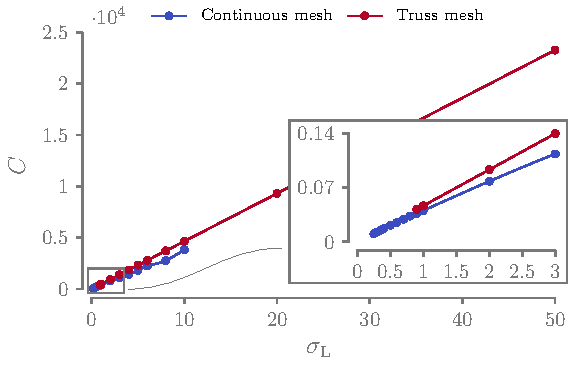
\includegraphics{figures/03_comparison_TO_TTO/14_stress_comp/stress_comp.pdf}
    \caption{Compliance $C$ versus maximum material allowable $\sigma_\text{L}$ plot for the density-based topology optimization and the \gls{tto} algorithms.}
    \label{fig:03_stress_comp}
\end{figure}

\figref{fig:03_stress_comp} depicts the compliance $C$ versus maximum material allowable $\sigma_\text{L}$ graph for the L-shaped beam test case. It is evident that the truss discretization of \gls{tto} consistently exhibits lower compliance values for every considered material allowable and maintains a perfectly linear relationship, in contrast to the continuous discretization approach. We speculate that the difference may be attributed to the more complex formulation (non-linearity, use of the filter, and projection), potentially causing the continuous approach to converge to a local minimum. It is worth noting that the differences between the two methods reduce for small $\sigma_\text{L}$ values.

\begin{marginfigure}
    Recall of \figref{fig:03_to_sol}c and d:
    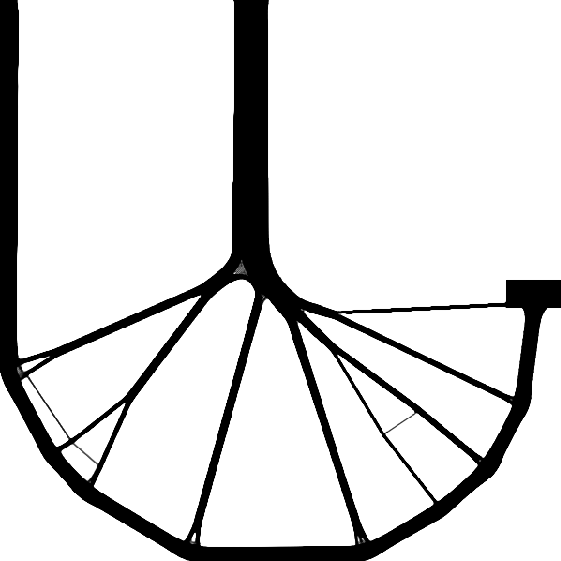
\includegraphics[width=0.8\linewidth]{figures/03_comparison_TO_TTO/07_to_sol/fig0_0.4.pdf}
\end{marginfigure}
\begin{marginfigure}
    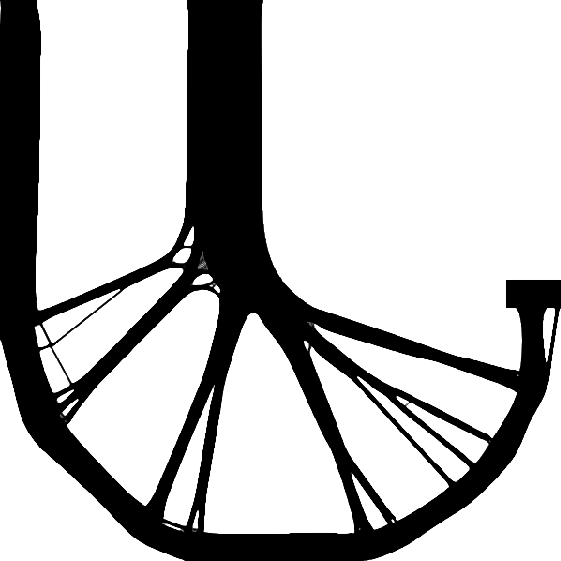
\includegraphics[width=0.8\linewidth]{figures/03_comparison_TO_TTO/07_to_sol/fig0_0.25.pdf}
\end{marginfigure}
In \figref{fig:03_stress_vol} we plot the different volume fractions obtained for a given material allowable (the axis in the graph are swapped as for us the most important figure of merit is the volume fraction).
\begin{figure}
    \centering
    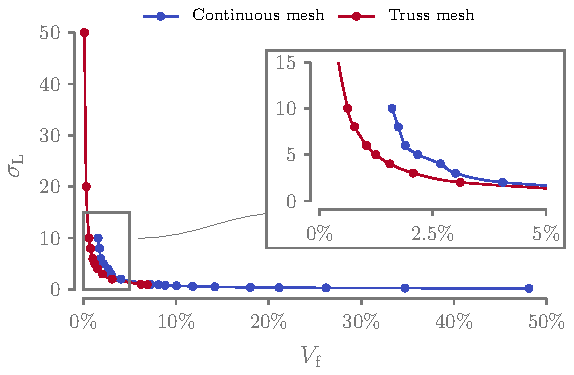
\includegraphics{figures/03_comparison_TO_TTO/15_stress_vol/stress_vol.pdf}
    \caption{Maximum material allowable $\sigma_\text{L}$ versus volume fraction $V_\text{f}$ plot for the density-based topology optimization and the \gls{tto} algorithms.}
    \label{fig:03_stress_vol}
\end{figure}
The density-based topology optimization yields structures that are more massive for a given material resistance. This outcome can be attributed not only to the aforementioned non-linearity in the formulation but also to another intriguing phenomenon. When dealing with high volume fractions (see \eg \figref{fig:03_to_sol}c and d), we observe that the material that composes the “beams” of the structure is distributed across multiple elements, appearing somewhat “smeared”. In contrast, the truss representation concentrates all the structural mass along the line extending from one node to another, putting the material exactly where needed and being, thus, numerically more efficient. This fact happens because the truss representation is an idealization, and it emphasizes the importance of ensuring that the chosen discretization remains within its applicable domain.

We can also observe that the truss representation serves as the lower limit of the topology optimization. We speculate that improving the convergence of the density-based topology optimization could potentially lead to results approaching those provided by the \gls{tto} algorithm. Interestingly, both discretizations follow a similar trend for high-volume fractions, despite the significant disparity in their physical description models. The very same trends can be observed watching the volume-complaince graph of \figref{fig:03_comp_vol}.
\begin{figure}
    \centering
    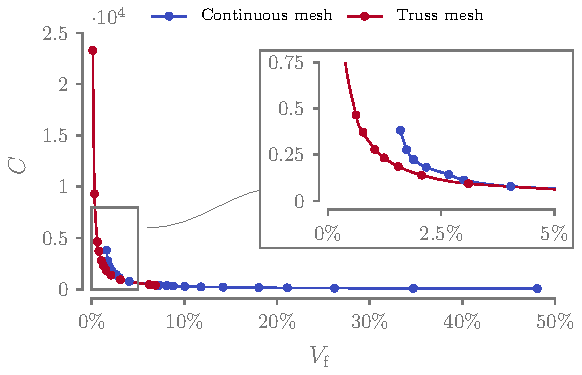
\includegraphics{figures/03_comparison_TO_TTO/16_comp_vol/comp_vol.pdf}
    \caption{Compliance $C$ versus volume fraction $V_\text{f}$ plot for the density-based topology optimization and the \gls{tto} algorithms.}
    \label{fig:03_comp_vol}
\end{figure}

Finally, in \figref{fig:03_time_vol} we turn our attention to the computational time comparison between the two optimization methods. It is noteworthy that a consistent three-order of magnitude difference is observed between the two methods (days vs. minutes) for every value of $V_\text{f}$. Additionally, it's worth recalling that for this specific test case, employing an extremely fine ground structure is not always a necessity, as we were able to obtain similar results (slightly more than \qty{1}{\percent} volume difference) with coarser ground structures (\qty{97}{\percent} fewer bars). This fact implies that the calculation time difference between density-based topology optimization and \gls{tto} could potentially be even bigger.

\begin{figure}
    \centering
    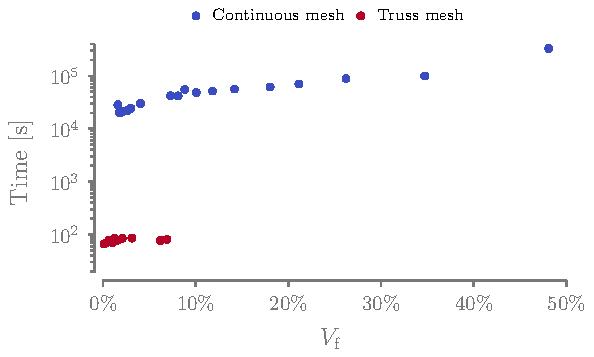
\includegraphics{figures/03_comparison_TO_TTO/17_time_vol/time_vol.pdf}
    \caption{Computational time $t$ versus volume fraction $V_\text{f}$ plot for the density-based topology optimization and the \gls{tto} algorithms.}
    \label{fig:03_time_vol}
\end{figure}

The notable difference in computation time for stress-based density-based topology optimization (which is not self-adjoint, in contrast to compliance minimization) points to the potential for exploring \gls{sand} approaches for density-based topology optimization. It's worth mentioning that \gls{sand} approaches typically lead to a substantial increase in the number of design variables\sidenote{In the \gls{sand} approach the displacements $\vect{u}$ are no more evaluated using the linear \gls{fem} equation $\matr{K}\vect{u}=\vect{f}$, but used as design variables of the optimization.}, but could beneficial when advanced mechanical constraints are used. In \gls{tto} problems, this is less of a concern due to the use of the ground structure approach, which results in numerous cross-sectional area design variables and fewer displacement-related ones. This, however, does not hold when dealing with a continuous mesh. While preliminary studies in this direction have been conducted~\sidecite{munro_local_2017}, they lie beyond the scope of this thesis and will not be further investigated. 

To sum up, the advantages of the \gls{tto} optimization algorithm become evident when considering the limitations of continuous discretization for optimizing ultralight structures. The first key drawback of density-based topology optimization is its increasing need for more elements to correctly discretize low-volume fraction structures, substantially augmenting computational time. Additionally, density-based topology optimization faces several numerical challenges, such as the need for constraint aggregation and relaxation. The optimization formulation proposed in this chapter addresses these problems but introduces another drawback: stress limit in optimized structures often exceed the specified allowable limit. To address this challenge, multiple approaches have been proposed within the aggregation framework to accurately account for the true constraint value, like using a set of active stress constraints~\sidecite{bruggi_topology_2012}, several aggregation clusters~\sidecite{paris_block_2010} or rectifier functions~\sidecite{norato_maximum-rectifier-function_2022}. However, all of these strategies come at the cost of increased computation time. Furthermore, stress constraints in continuous discretization are often defined for equivalent von Mises stress, making it more challenging to distinguish between asymmetric bounds for tension and compression. New failure criteria should then be implemented. Finally, the optimization of ultralight structures naturally tends to result in truss-like topologies regardless of the chosen optimization formulation. These structures are naturally subject to local buckling as a mode of failure~\sidecite{sigmund_non-optimality_2016}, a phenomenon that is difficult to describe when using continuous elements.

While truss discretization offers advantages in terms of computational efficiency, it does come with certain limitations. In the minimum volume formulation, the problem is linear and cost-effective to solve. However, the linearity is lost when additional constraints, such as local buckling, are introduced. Moreover, as the \gls{fem} equation $\matr{K}\vect{u}=\vect{f}$ is never explicitly solved during the optimization, the \gls{sand} formulation does not inherently account for the kinematic compatibility of the displacements and the forces of the problem. This limitation restricts its applicability to relatively simple problems, such as those presented in this chapter, where kinematic compatibility was inherently satisfied. Issues can arise, however, when dealing with complex scenarios involving multiple loads or constraints that may lead to statically indeterminate structures. These limitations are well-known in the literature of \gls{tto} and should be taken into account during the optimization if we decide to pursue the development of the optimization algorithm using the \gls{tto} framework.

\section{Conclusion}
Since the first developments of the topology optimization method, it has been recognized that "For moderately low volume fractions the lay-out of truss-like structures is predicted, but for very low volume fractions it is recommended that the traditional layout theory be employed..."~\sidecite{bendsoe_optimal_1989}. However, the performance gap has never been quantified, nor has the domain of applicability been assessed. Additionally, it's important to note that these assumptions were primarily based on compliance formulations and not on volume minimization formulations, which are more pertinent to the aeronautical context.

In this chapter, we assessed the suitability of employing the \gls{tto} algorithm for the optimization of ultralight structures by quantifying the disparities between density-based topology optimization and \gls{tto} under the volume minimization under strength constraints formulation. We introduced a standardized two-dimensional test case, the L-shaped beam, commonly utilized in stress-based optimization scenarios. Multiple optimization runs are conducted for both discretization methods, employing various materials, and the results are subsequently compared, with a primary focus on volume fraction, compliance, stress, and computational time in the optimized structures.

Considering the limitations encountered with the continuous approach, particularly at very low volume fractions, we opted to pursue our optimization algorithm development using the \acrfull{tto} framework. The use of a ground structure to discretize the design space is more coherent with the type of structures we are working on, and the use of the \gls{sand} approach permits us to drastically reduce the computational time and take into account additional constraints more easily \marginnote{The sensitivity calculation is easier, as the different design variables are not explicitly dependent on each other.}. We also identified certain limitations inherent to truss discretizations, namely the need to take into account the kinematic compatibility of the structure and the local buckling failure mode, which will be addressed in the following chapter.